\subsection{Tutorial}
Il tutorial di seguito è possibile anche trovarlo al link: \href{https://github.com/Wabri/ATTSW_Exam/blob/master/gradle.example/third/}{\textsc{github.com/Wabri/ATTSW\_Exam/blob/master/gradle.example/third/}}.
\begin{enumerate}
    \item Creare una cartella gradle.example/third
    \item Eseguire la build:
\begin{verbatim}
    $ gradle init --type java-application
\end{verbatim}
    \item Controllare e nel caso modificare il build.gradle per fare in modo di avere:
    \begin{itemize}
        \item il java plugin
        \item Come unica repository MavenCentral
        \item junit 4.12
    \end{itemize}
    \item Eseguire la build \texttt{dependencies} per scaricare le dipendenze
    \item Assicurarsi che junit sia configurato per il testImplementation, com'è possibile notare dal comando precedente la configurazione testCompile è deprecata
    \item Eseguire nuovamente la build \texttt{dependencies}, controllare se la dipendenza junit è stata associata alla configurazione testImplementation
    \item Eseguire la build di test con continuous:
    \begin{verbatim}
    $ ./gradlew test --continuous\end{verbatim}
    \item Aggiungere il metodo helloWorldSendTest nella classe di test AppTest:
    \begin{lstlisting}[frame=single]
    @Test 
    public void helloWorldSendTest () {
	    App classUnderTest = new App();
	    assertEquals("Hello world!", classUnderTest.getGreeting());
    }
    \end{lstlisting}
    Questo dovrà far fallire la build test avviata nel punto precedente.
    \item Correggere il test modificando il metodo getGreeting() nella classe App:
    \begin{lstlisting}[frame=single]
    public String getGreeting() {
        return "Hello world!";
    }
    \end{lstlisting}
    A questo punto la build test avrà successo.
    \item Stoppare la build test usando la combinazione \texttt{ctrl+d}
    \item Eseguire la build di test con continuous sul metodo testAppHasAGreeting():
    \begin{verbatim}
    $ ./gradlew test --continuous --tests AppTest.testAppHasAGreeting \end{verbatim}
    \item Modificare il metodo di test helloWorldSendTest:
    \begin{lstlisting}[frame=single]
    @Test 
    public void helloWorldSendTest () {
	    App classUnderTest = new App();
	    assertEquals("Greetings", classUnderTest.getGreeting());
    }
    \end{lstlisting}
    Ovviamente la build avrà successo dato che non stiamo modificando il metodo sotto test. Stoppare quindi la build usando \texttt{ctrl+d}
    \item Modificare il metodo getGreeting della classe App in modo da non far fallire la build:
    \begin{verbatim}
    $ ./gradlew test --continuous --tests \*Test\end{verbatim}
    \item Aggiungere il MANIFEST alla build.gradle:
    \begin{lstlisting}[frame=single]
    jar {
        manifest {
            attributes("Implementation-Title": "App","Implementation-Version":1.0,'Main-Class':'App')
        }
    }
    \end{lstlisting}
    \item Eseguire la build jar:
    \begin{verbatim}
        $ ./gradlew jar\end{verbatim}
    \item Provare ad eseguire l'applicativo appena creato (che si troverà nella directory build/libs/):
    \begin{verbatim}
        $ java -jar build/libs/third.jar \end{verbatim}
    Quello che dovrà comparire sarà la stringa di ritorno del metodo getGreeting().
    \item Aggiungere alla lista dei plugin quello di eclipse:
    \begin{lstlisting}[frame=single]
    id 'eclipse'
    \end{lstlisting}
    \item Eseguire la build di creazione metadati di eclipse:
    \begin{verbatim}
        $ ./gradlew eclipse \end{verbatim}
    \item Importare il progetto su eclipse:
    \begin{figure}[H]
        \begin{subfigure}{0.5\textwidth}
        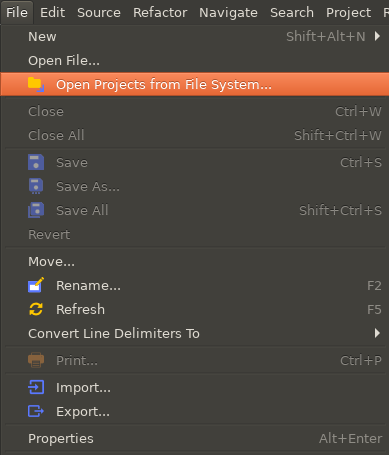
\includegraphics[width=1.0\linewidth, height=7cm]{3DependencyManagement/tutorial/importProject.png}
        \end{subfigure}
        \begin{subfigure}{0.5\textwidth}
        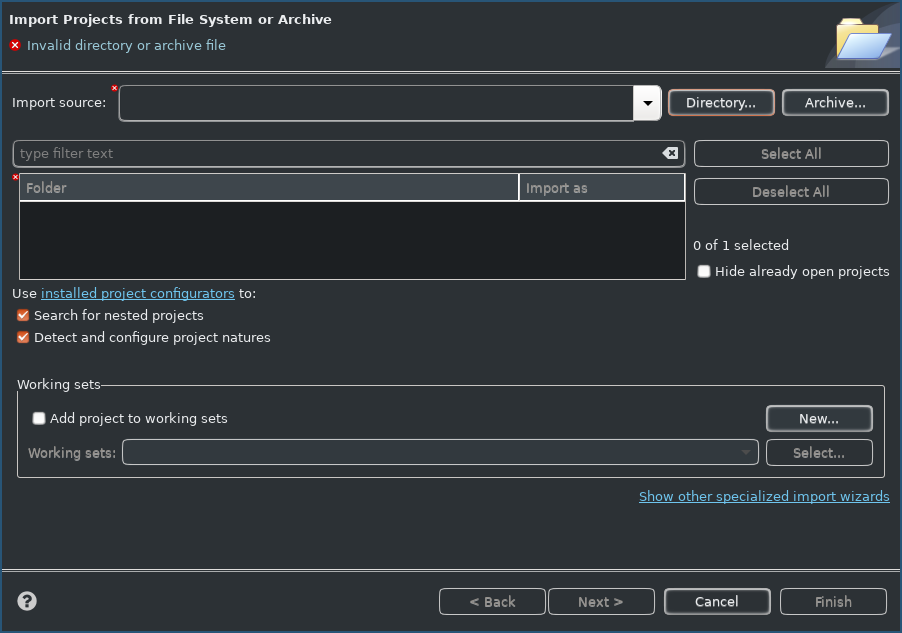
\includegraphics[width=1.0\linewidth, height=7cm]{3DependencyManagement/tutorial/importSource.png}
        \end{subfigure}
    \end{figure}
    \item Eseguire la build \texttt{test} usando la view \texttt{Gradle Tasks} di Eclipse
    \item Se la build di test è andata a buon fine allora eseguire la build \texttt{jar}, sempre usando il \texttt{Gradle Tasks}
    \item Testare il funzionamento dell'ultima build eseguendo da terminale il solito comando del punto 16
\end{enumerate}